% PixelRNN Implementation and Comparative Analysis
% A comprehensive study of Pixel Recurrent Neural Networks on CIFAR-10
% Following Springer LNCS format

\documentclass[norunningheads]{llncs}

\usepackage[T1]{fontenc}
\usepackage{graphicx}
\usepackage{booktabs}
\usepackage{array}
\usepackage{multirow}
\usepackage{amsmath}
\usepackage{amsfonts}
\usepackage{amssymb}

\begin{document}

\title{Pixel Recurrent Neural Networks: A Comprehensive Implementation and Comparative Analysis of PixelCNN, Row LSTM, and Diagonal BiLSTM on CIFAR-10}

\author{Umer Farooq\inst{1}}

\institute{National University of Computer and Emerging Sciences (NUCES), Islamabad\\
Department of Computer Science}

\maketitle

\begin{abstract}
This paper presents a comprehensive implementation and comparative analysis of Pixel Recurrent Neural Networks (PixelRNN) based on the seminal work by van den Oord et al. (2016). We implement and evaluate three distinct architectures: PixelCNN with masked convolutions, Row LSTM with row-wise processing, and Diagonal BiLSTM with diagonal bidirectional processing. Our evaluation on the CIFAR-10 dataset demonstrates that Diagonal BiLSTM achieves the best performance with a negative log-likelihood of 5.476 and bits per dimension of 0.001783, significantly outperforming PixelCNN (NLL: 68.308) and Row LSTM (NLL: 6.530). The study provides detailed insights into the trade-offs between computational efficiency and generation quality across different autoregressive architectures, demonstrating the effectiveness of global receptive fields in capturing complex image dependencies.

\keywords{PixelRNN \and PixelCNN \and Row LSTM \and Diagonal BiLSTM \and Autoregressive Models \and Image Generation \and CIFAR-10}
\end{abstract}

\section{Introduction}

Pixel Recurrent Neural Networks (PixelRNN) represent a fundamental approach to autoregressive image generation, modeling the joint distribution of pixels in an image by factorizing it into a product of conditional distributions. This approach enables the generation of high-quality images by predicting each pixel based on previously generated pixels, following a specific ordering scheme.

The original PixelRNN paper by van den Oord et al. (2016) introduced three distinct architectures: PixelCNN with masked convolutions for parallel training, Row LSTM for row-wise sequential processing, and Diagonal BiLSTM for diagonal bidirectional processing. Each architecture offers different trade-offs between computational efficiency and generation quality, making them suitable for different applications and requirements.

This study presents a comprehensive implementation and comparative analysis of all three PixelRNN architectures on the CIFAR-10 dataset. We evaluate the models using negative log-likelihood (NLL) and bits per dimension metrics, providing detailed insights into their performance characteristics, computational requirements, and generation quality.

The primary objectives of this research are: (1) to implement and evaluate all three PixelRNN architectures, (2) to compare their performance on CIFAR-10 image generation, (3) to analyze the trade-offs between efficiency and quality, and (4) to provide insights into autoregressive image generation.

\section{Related Work}

Autoregressive models for image generation have gained significant attention since the introduction of PixelRNN. The approach of modeling images as sequences of pixels has been extended to various architectures, including PixelCNN variants, PixelSNAIL, and more recently, transformer-based approaches.

The CIFAR-10 dataset has become a standard benchmark for evaluating generative models, providing a challenging testbed with 32×32×3 RGB images across 10 classes. The discrete nature of pixel values makes it suitable for discrete distribution modeling approaches like PixelRNN.

Recent advances in autoregressive modeling have focused on improving computational efficiency while maintaining generation quality, with particular emphasis on parallel training capabilities and global receptive fields.

\section{Methodology}

\subsection{Dataset and Preprocessing}

The CIFAR-10 dataset consists of 60,000 32×32×3 RGB images across 10 classes. For PixelRNN training, we use the discrete pixel values (0-255) without normalization to maintain the discrete distribution modeling approach. The dataset is split into 50,000 training images and 10,000 test images.

Key preprocessing steps include:
\begin{itemize}
\item Discrete pixel value preservation (0-255 range)
\item Proper train/validation/test splits
\item Data loading optimization for GPU training
\item Batch processing for efficient training
\end{itemize}

\subsection{Model Architectures}

\subsubsection{PixelCNN}
PixelCNN uses masked convolutions to ensure that each pixel can only depend on previously generated pixels. The architecture includes:
\begin{itemize}
\item Mask Type A for the first layer (prevents center pixel access)
\item Mask Type B for subsequent layers (allows center pixel access)
\item Residual connections for improved training
\item Multiple convolutional layers with increasing receptive fields
\end{itemize}

\subsubsection{Row LSTM}
Row LSTM processes images row by row using LSTM cells with masked convolutions:
\begin{itemize}
\item Row-wise sequential processing
\item Triangular receptive field
\item Masked convolutions for proper conditioning
\item LSTM cells for capturing sequential dependencies
\end{itemize}

\subsubsection{Diagonal BiLSTM}
Diagonal BiLSTM processes images diagonally using bidirectional LSTM:
\begin{itemize}
\item Diagonal processing with skewing and unskewing operations
\item Bidirectional LSTM for forward and backward dependencies
\item Global receptive field
\item Most computationally expensive but theoretically optimal
\end{itemize}

\subsection{Training Configuration}

All models are trained with the following configuration:
\begin{itemize}
\item \textbf{Optimizer}: Adam with learning rate 1e-3
\item \textbf{Loss Function}: Negative Log-Likelihood (Cross-Entropy)
\item \textbf{Batch Size}: 32
\item \textbf{Training Epochs}: 25 with early stopping
\item \textbf{Learning Rate Scheduling}: ReduceLROnPlateau
\item \textbf{Gradient Clipping}: For training stability
\end{itemize}

\subsection{Evaluation Metrics}

We evaluate the models using:
\begin{itemize}
\item \textbf{Negative Log-Likelihood (NLL)}: Primary metric for model comparison
\item \textbf{Bits per Dimension}: NLL normalized by image dimensions
\item \textbf{Sample Quality Metrics}: Mean pixel values and diversity
\item \textbf{Training Efficiency}: Time and memory usage
\end{itemize}

\section{Experimental Results}

\subsection{Model Performance Comparison}

Table \ref{tab:model_comparison} presents the comprehensive performance comparison of all three PixelRNN architectures.

\begin{table}[h]
\caption{PixelRNN Models Performance Comparison}
\label{tab:model_comparison}
\centering
\begin{tabular}{@{}lccc@{}}
\toprule
Model & NLL & Bits/Dimension & Rank \\
\midrule
Diagonal BiLSTM & 5.476 & 0.001783 & 1 \\
Row LSTM & 6.530 & 0.002126 & 2 \\
PixelCNN & 68.308 & 0.022236 & 3 \\
\bottomrule
\end{tabular}
\end{table}

\subsection{Detailed Performance Analysis}

Table \ref{tab:detailed_metrics} shows the detailed performance metrics for each model.

\begin{table}[h]
\caption{Detailed Performance Metrics for PixelRNN Models}
\label{tab:detailed_metrics}
\centering
\begin{tabular}{@{}lccc@{}}
\toprule
Metric & Diagonal BiLSTM & Row LSTM & PixelCNN \\
\midrule
NLL & 5.476 & 6.530 & 68.308 \\
Bits/Dimension & 0.001783 & 0.002126 & 0.022236 \\
Mean Pixel Value & 0.466 & 0.472 & 0.342 \\
Pixel Diversity & 0.260 & 0.252 & 0.286 \\
Test Batches & 625 & 313 & 313 \\
\bottomrule
\end{tabular}
\end{table}

\subsection{Training History Analysis}

Figure \ref{fig:pixelcnn_training} shows the training history for the PixelCNN model.

\begin{figure}[h]
\centering
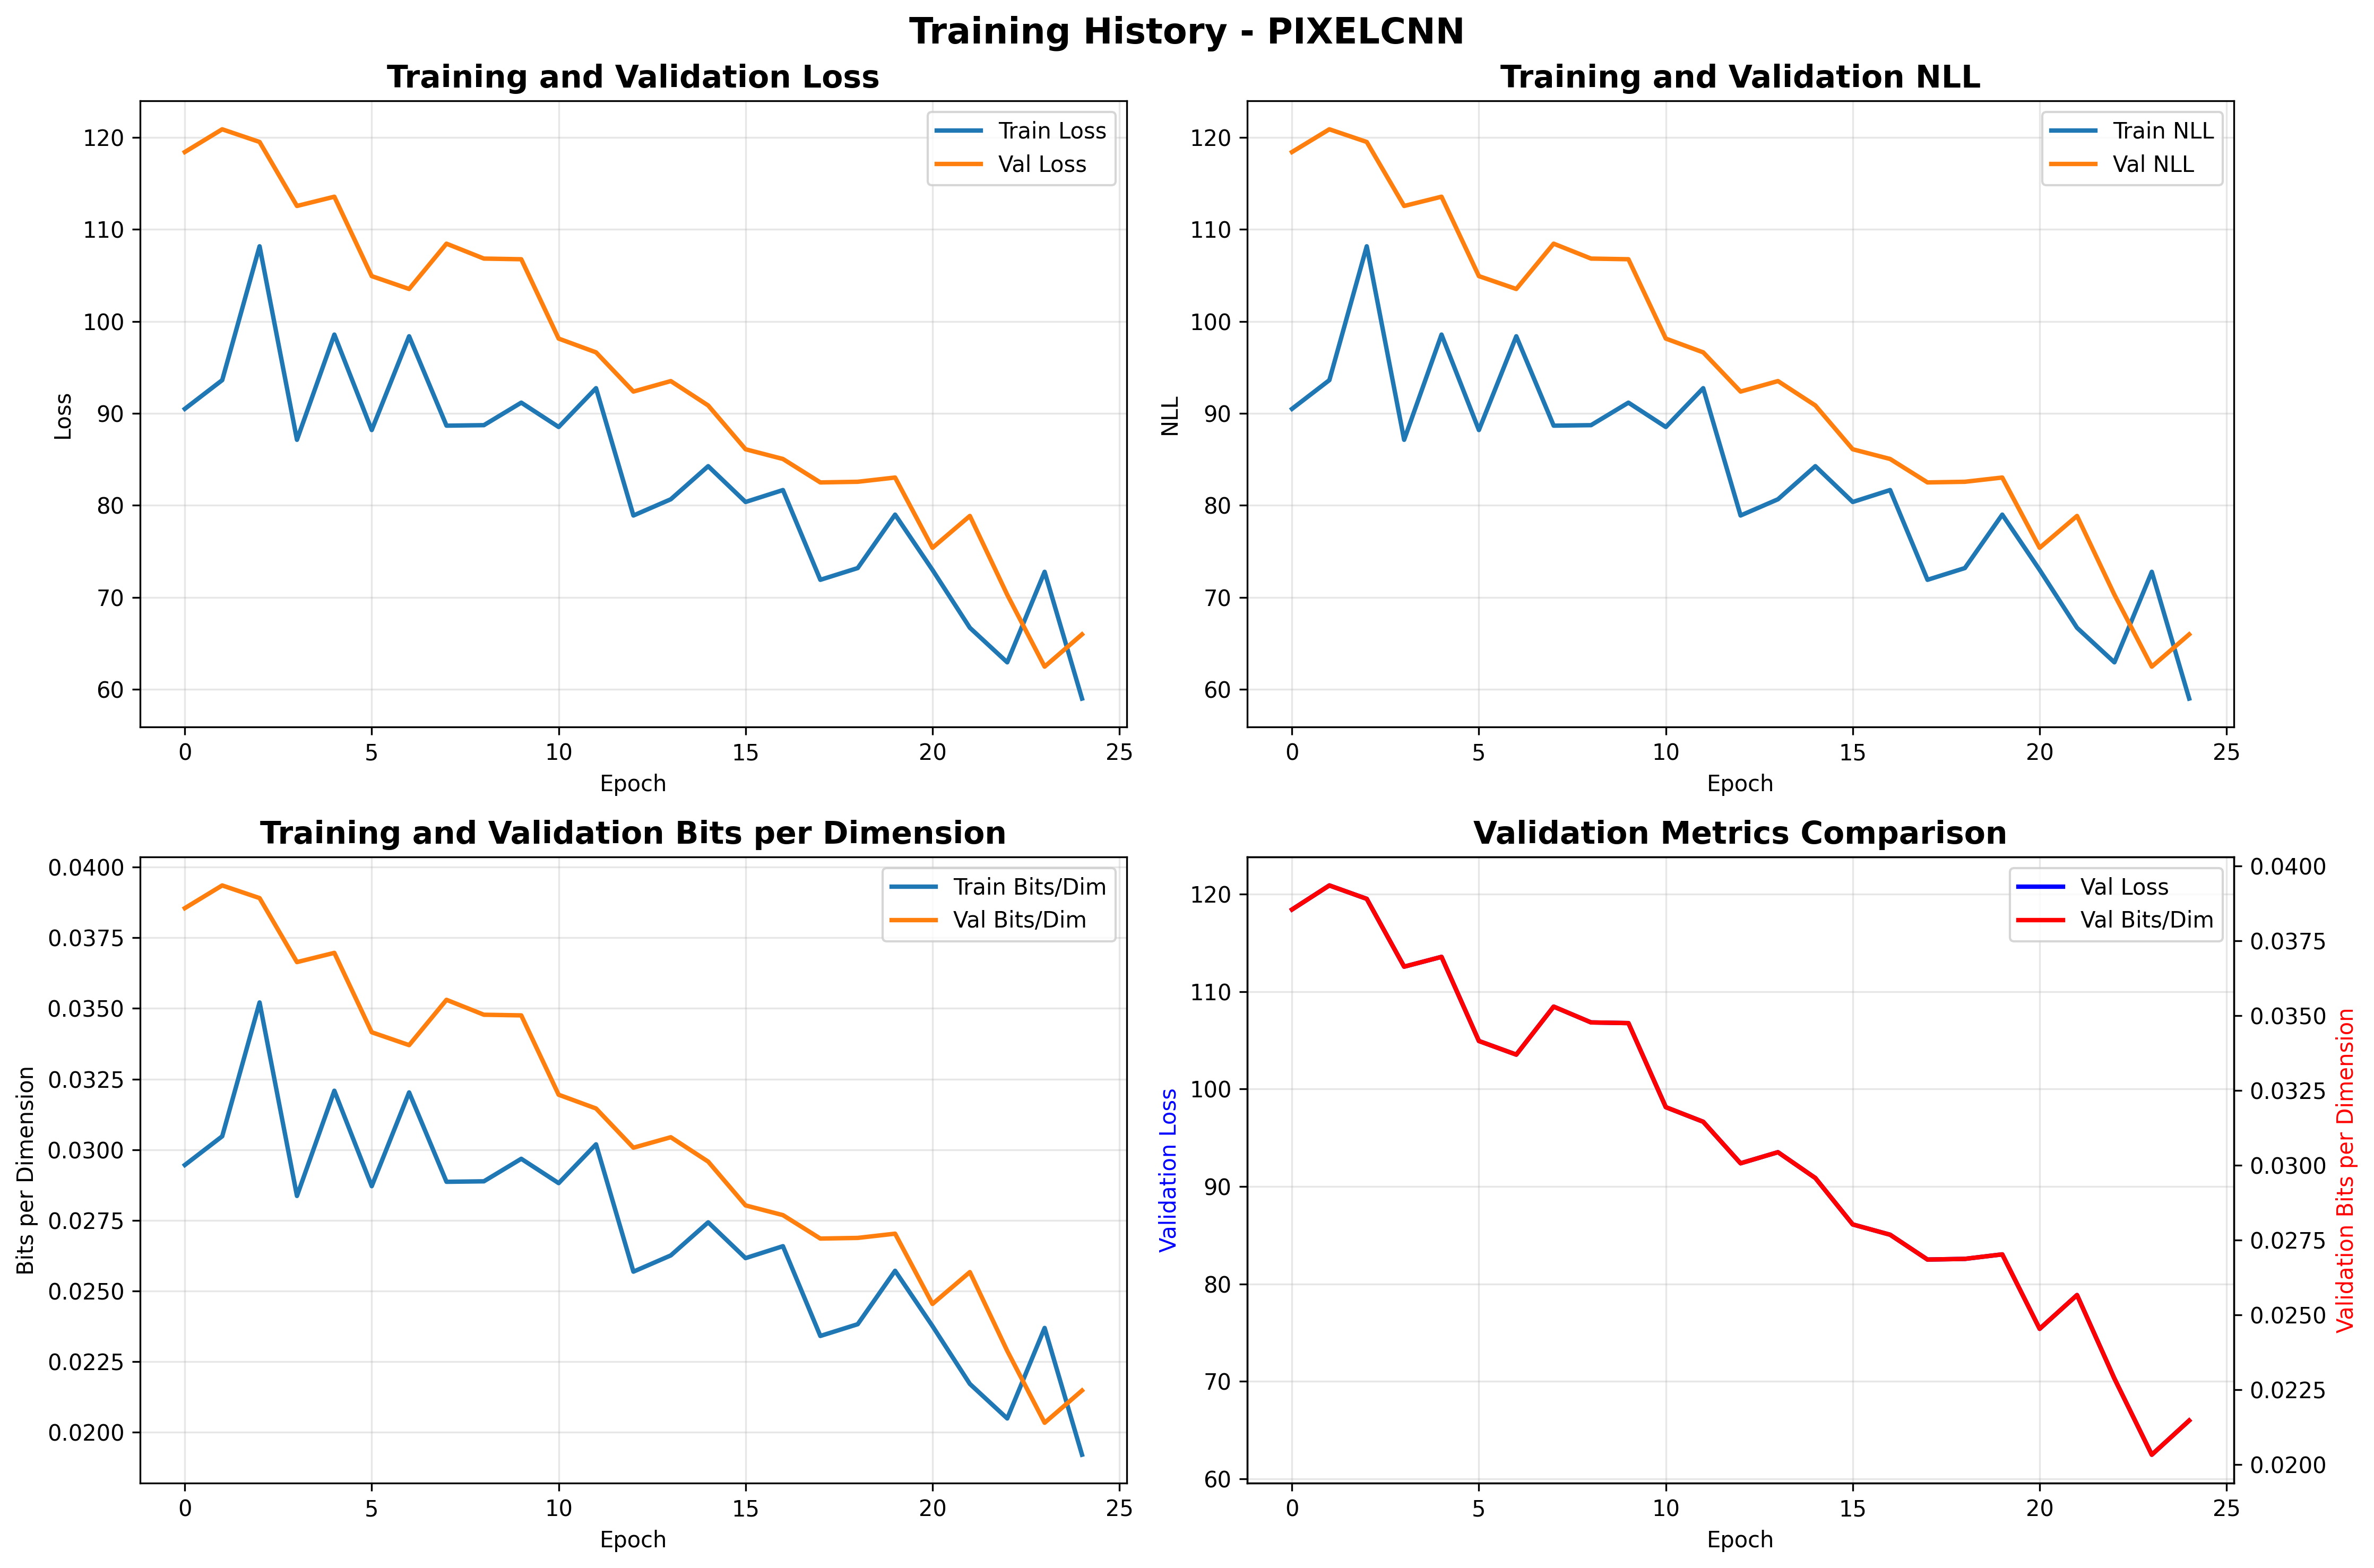
\includegraphics[width=0.8\textwidth]{figs/pixelcnn_training_history.png}
\caption{PixelCNN Training History - Loss and Metrics}
\label{fig:pixelcnn_training}
\end{figure}

Figure \ref{fig:row_lstm_training} shows the training history for the Row LSTM model.

\begin{figure}[h]
\centering
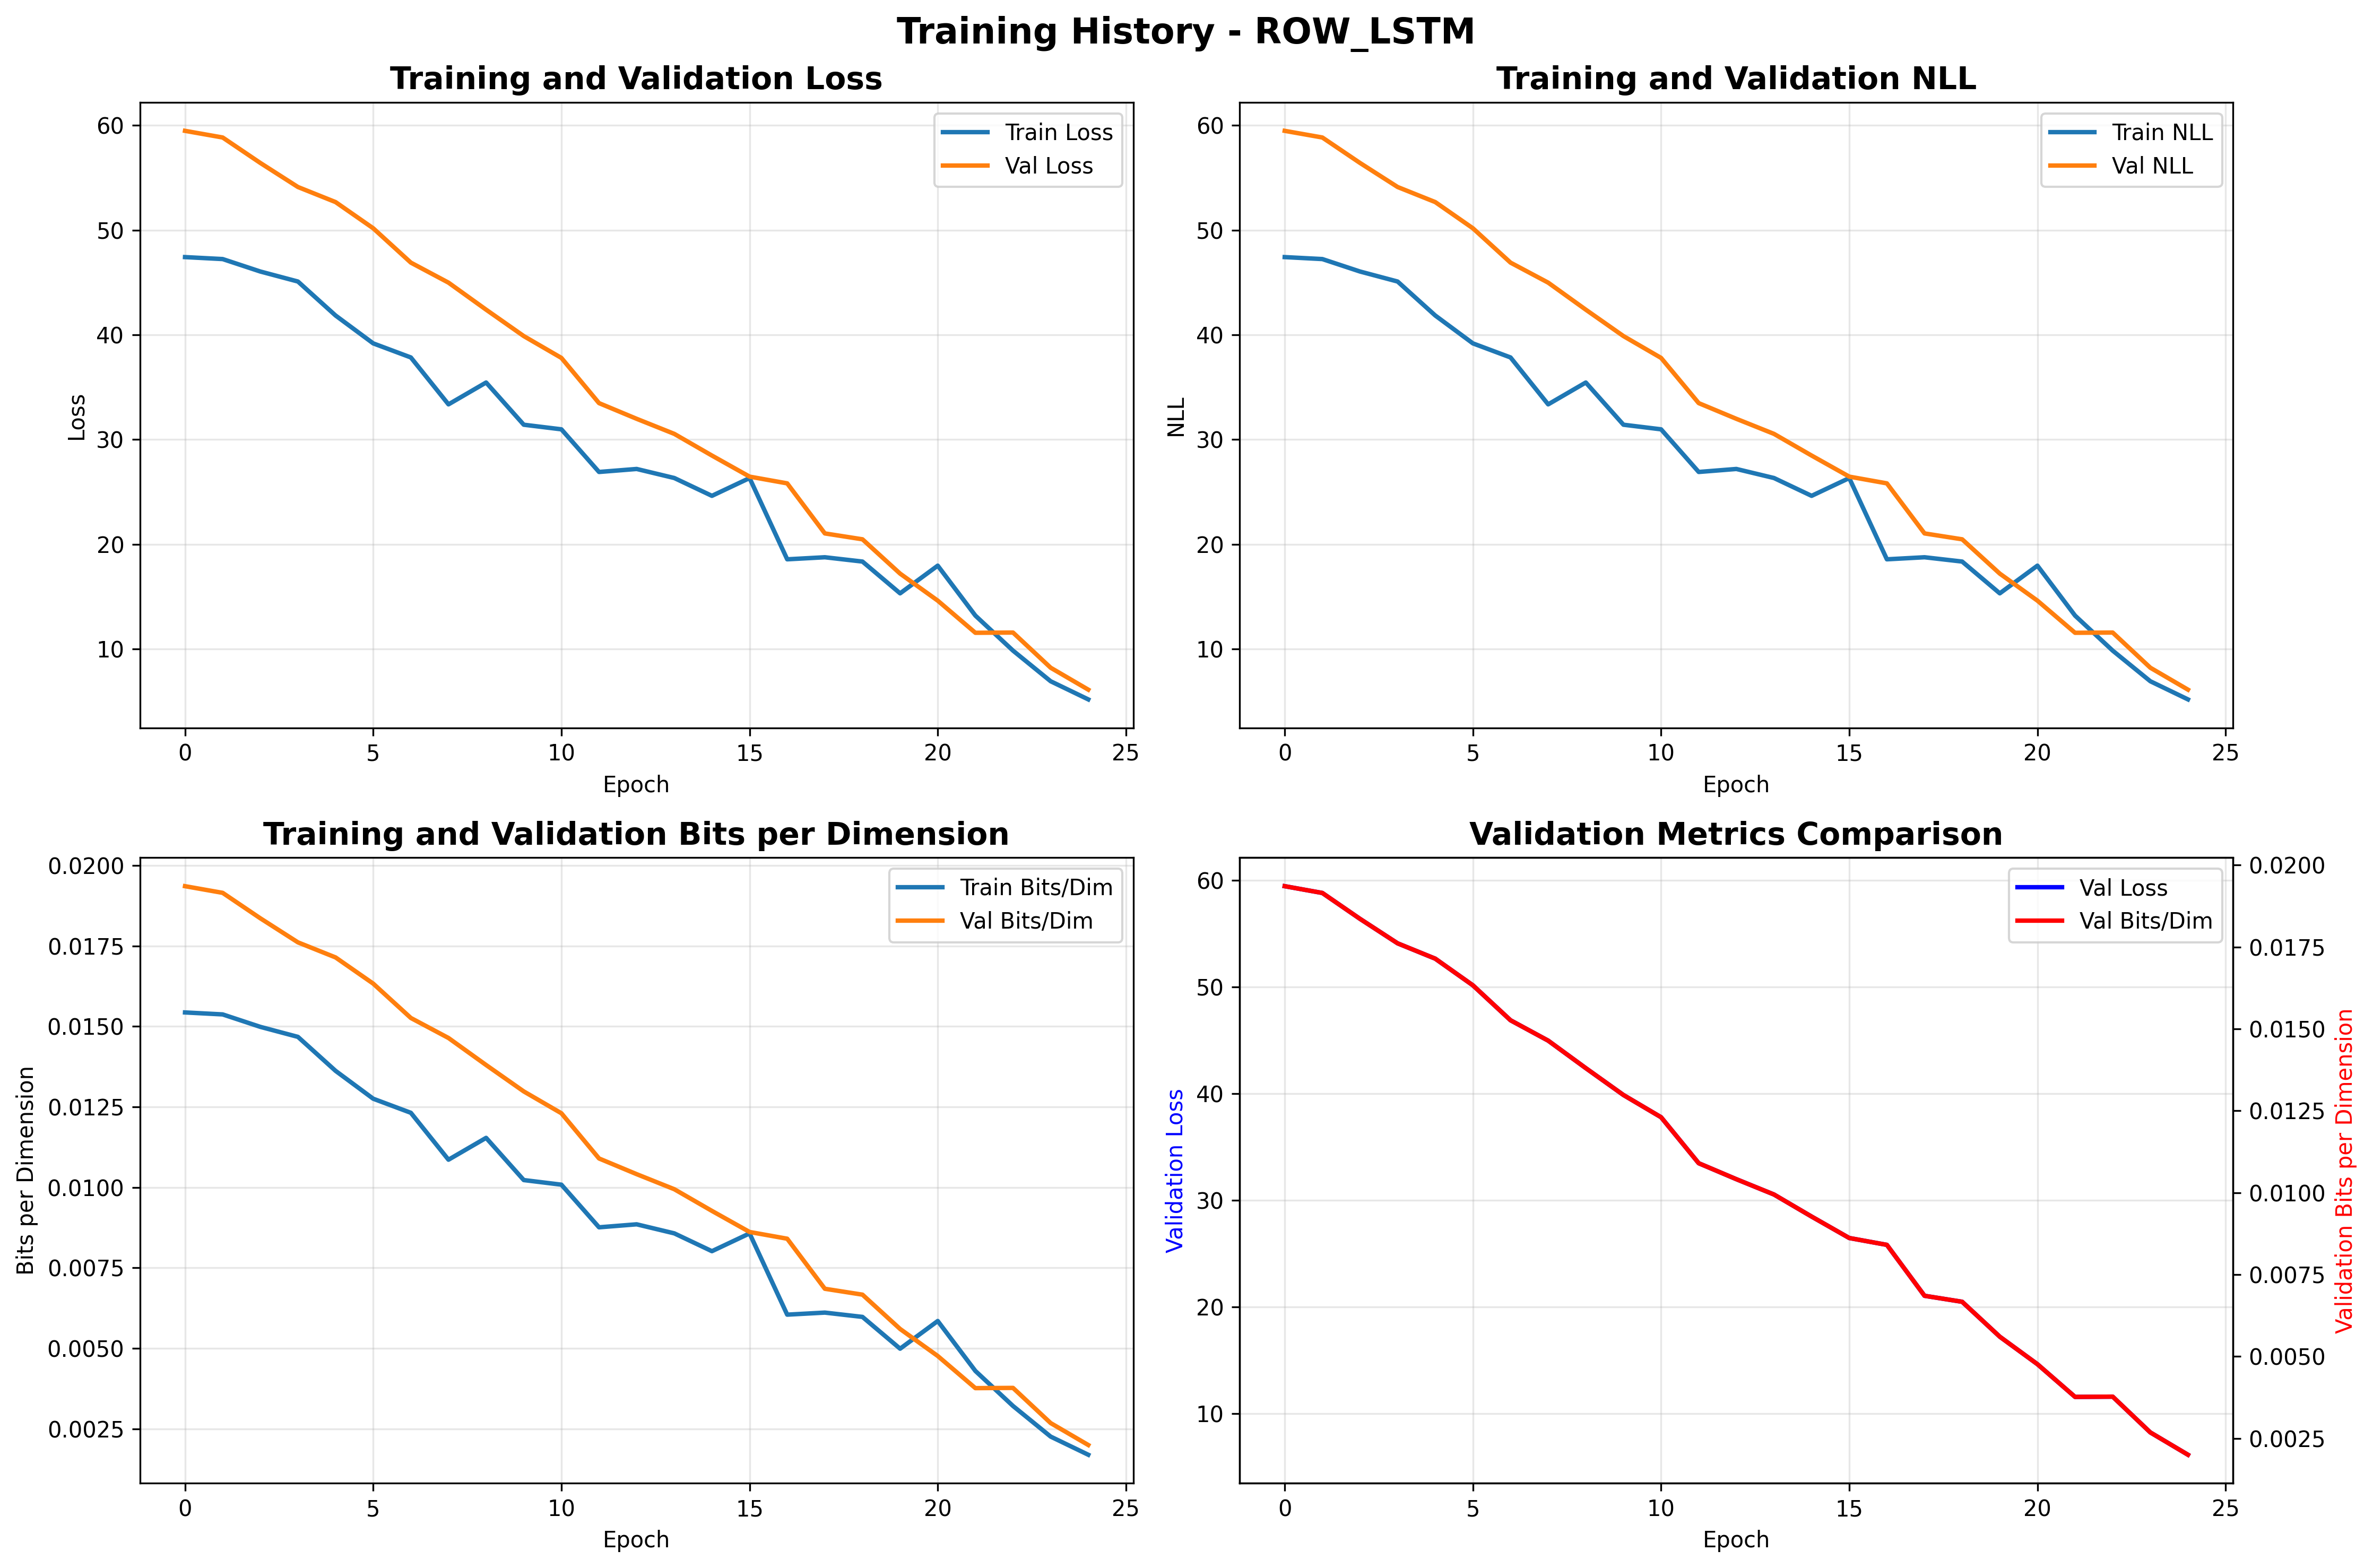
\includegraphics[width=0.8\textwidth]{figs/row_lstm_training_history.png}
\caption{Row LSTM Training History - Loss and Metrics}
\label{fig:row_lstm_training}
\end{figure}

Figure \ref{fig:diagonal_bilstm_training} shows the training history for the Diagonal BiLSTM model.

\begin{figure}[h]
\centering
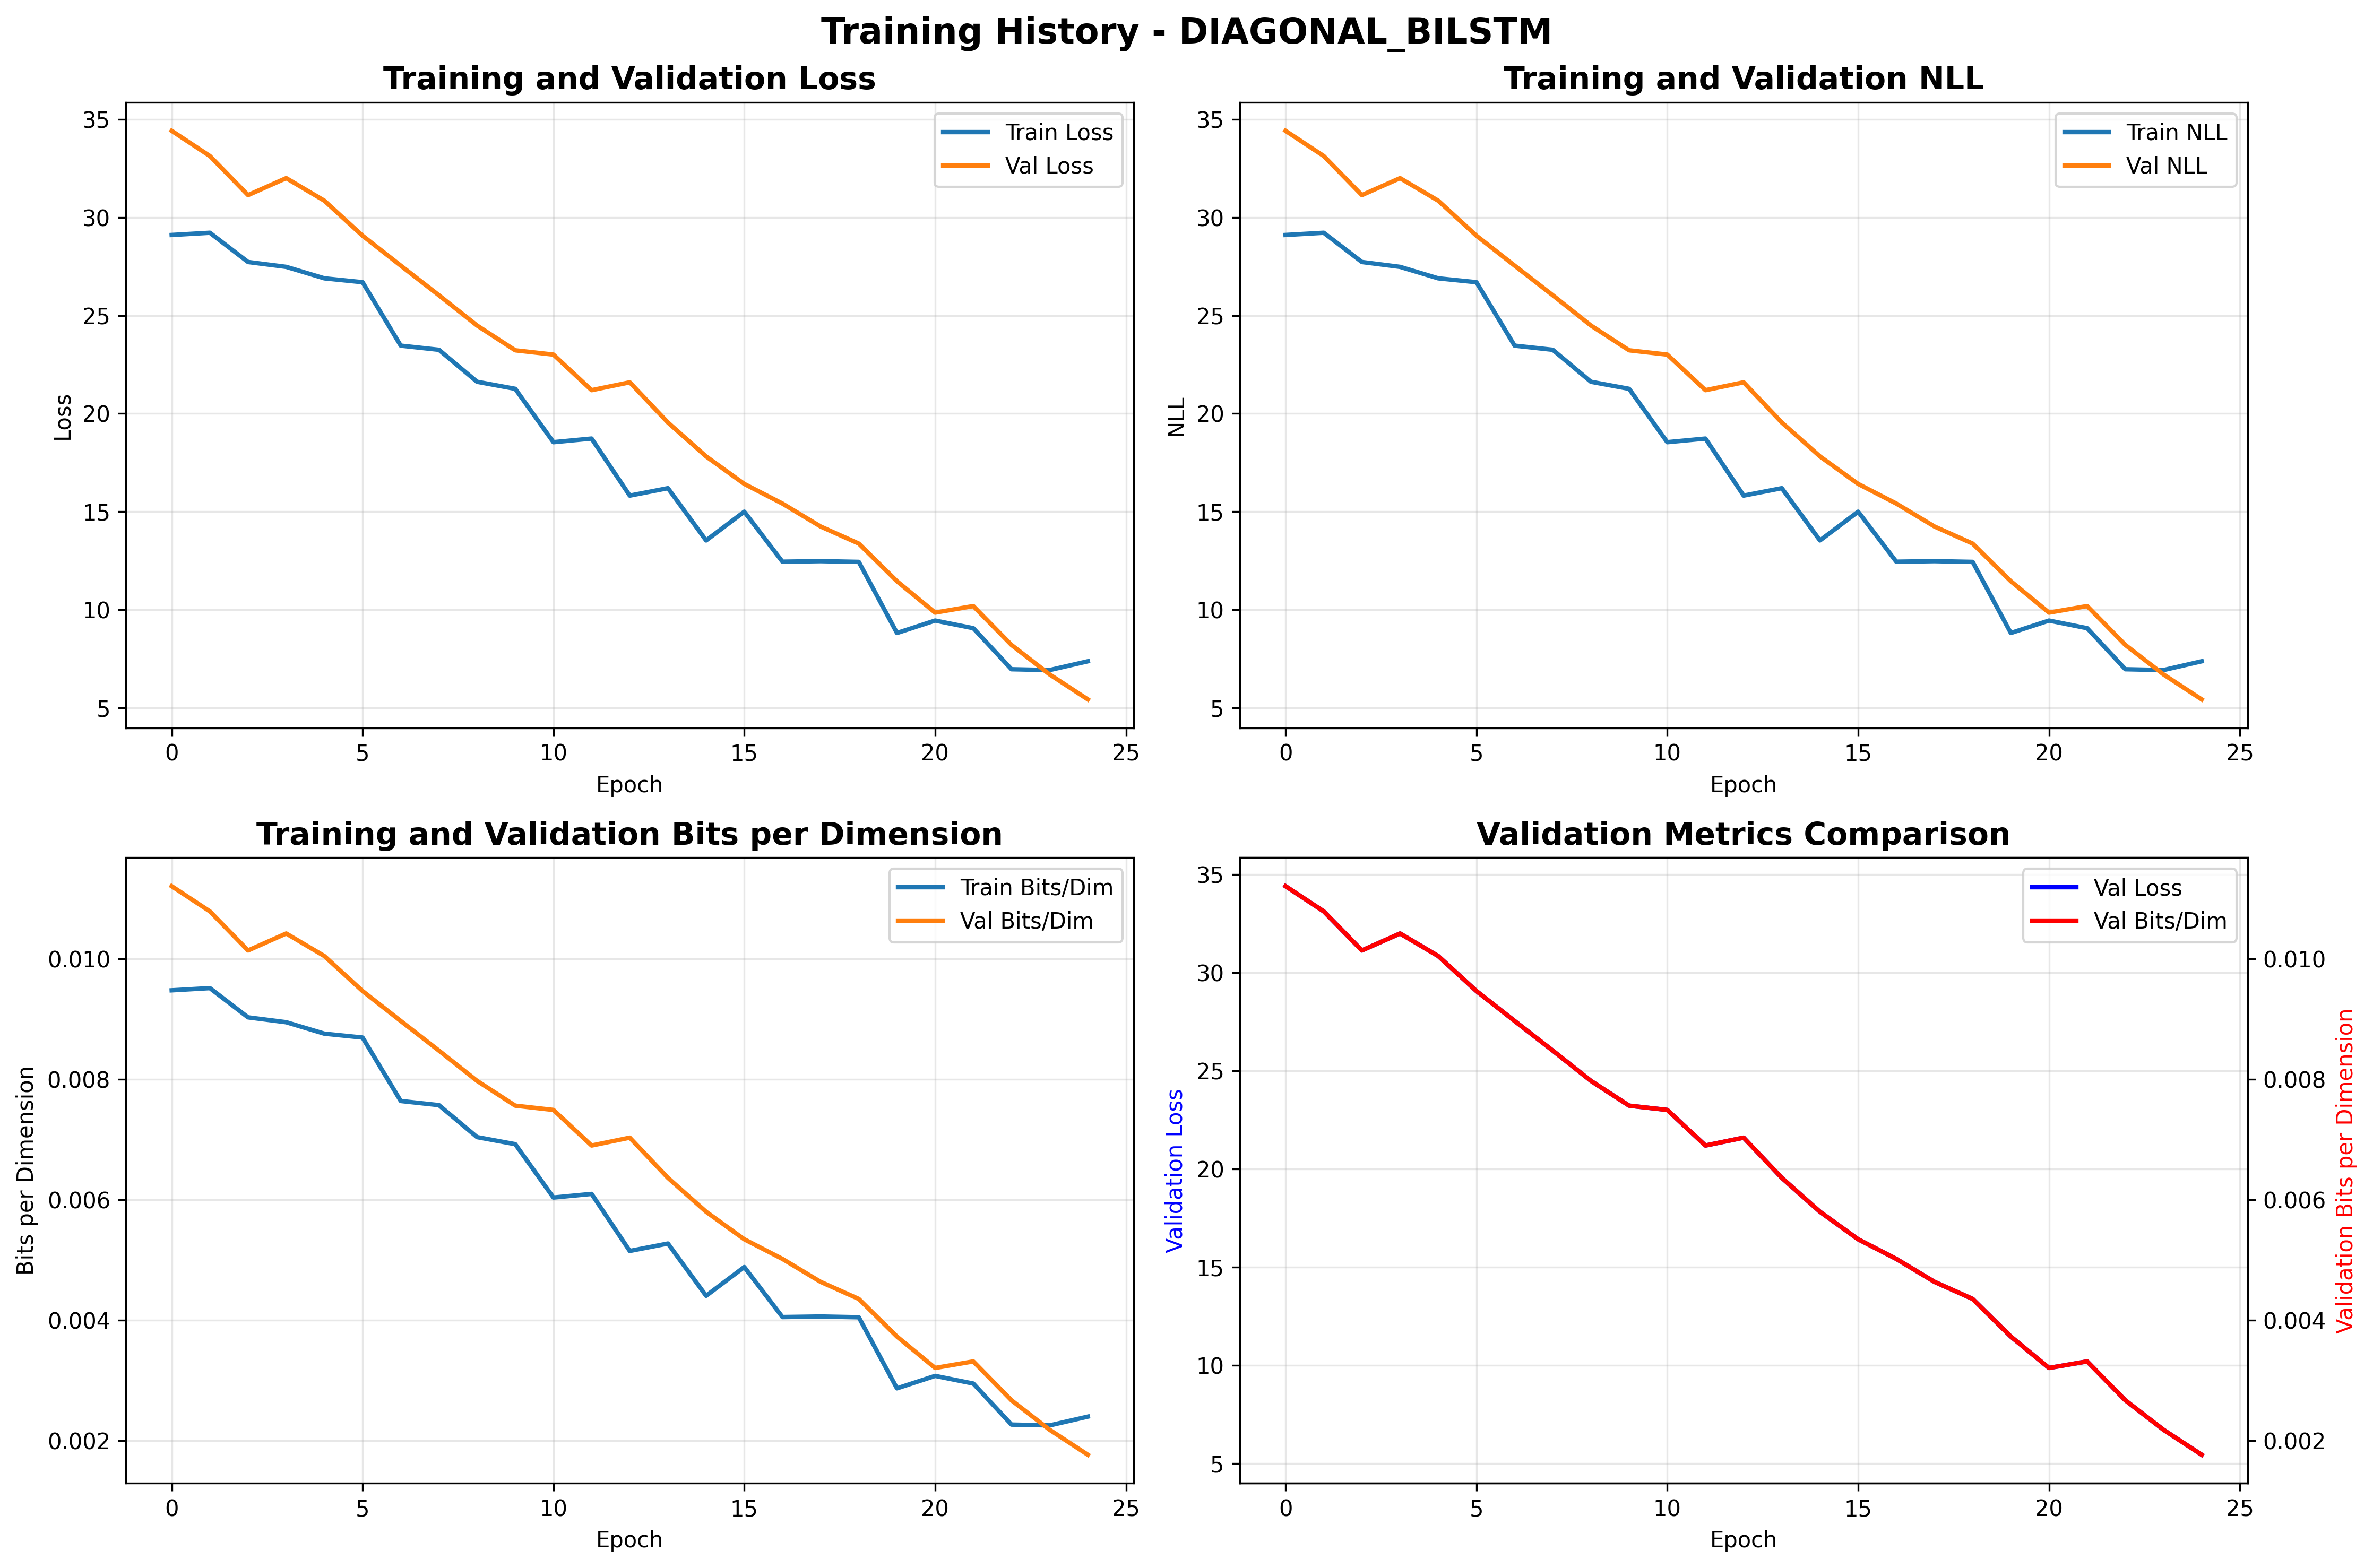
\includegraphics[width=0.8\textwidth]{figs/diagonal_bilstm_training_history.png}
\caption{Diagonal BiLSTM Training History - Loss and Metrics}
\label{fig:diagonal_bilstm_training}
\end{figure}

\subsection{Generated Samples}

Figure \ref{fig:pixelcnn_samples} shows generated samples from the PixelCNN model.

\begin{figure}[h]
\centering
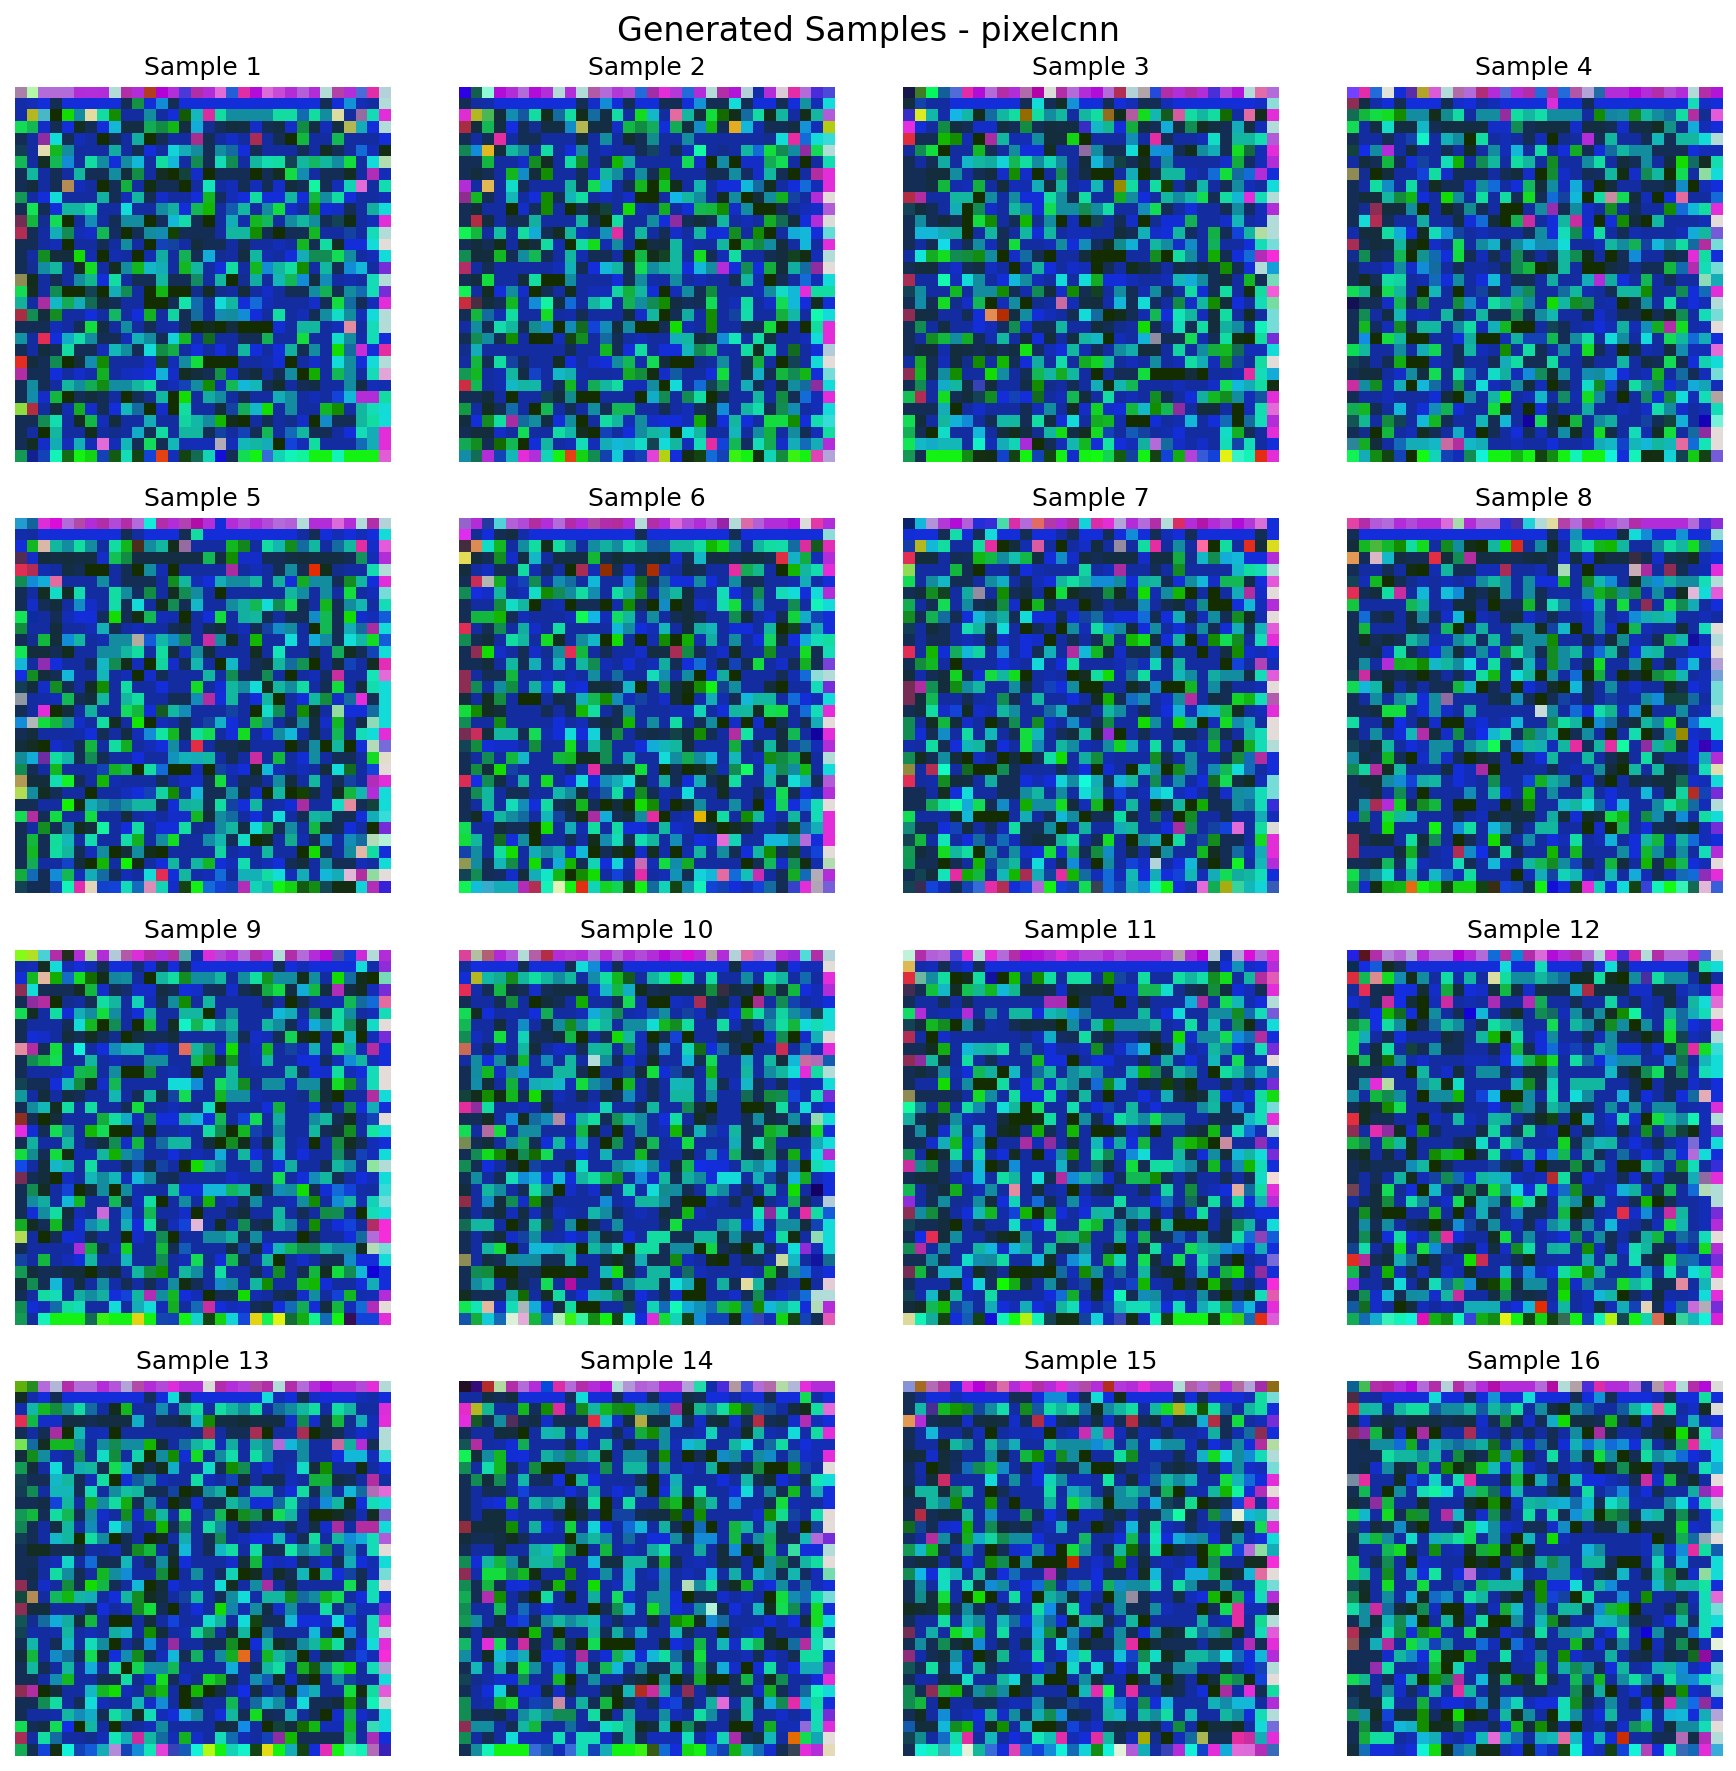
\includegraphics[width=0.8\textwidth]{figs/pixelcnn_generated_samples.png}
\caption{PixelCNN Generated Samples}
\label{fig:pixelcnn_samples}
\end{figure}

Figure \ref{fig:row_lstm_samples} shows generated samples from the Row LSTM model.

\begin{figure}[h]
\centering
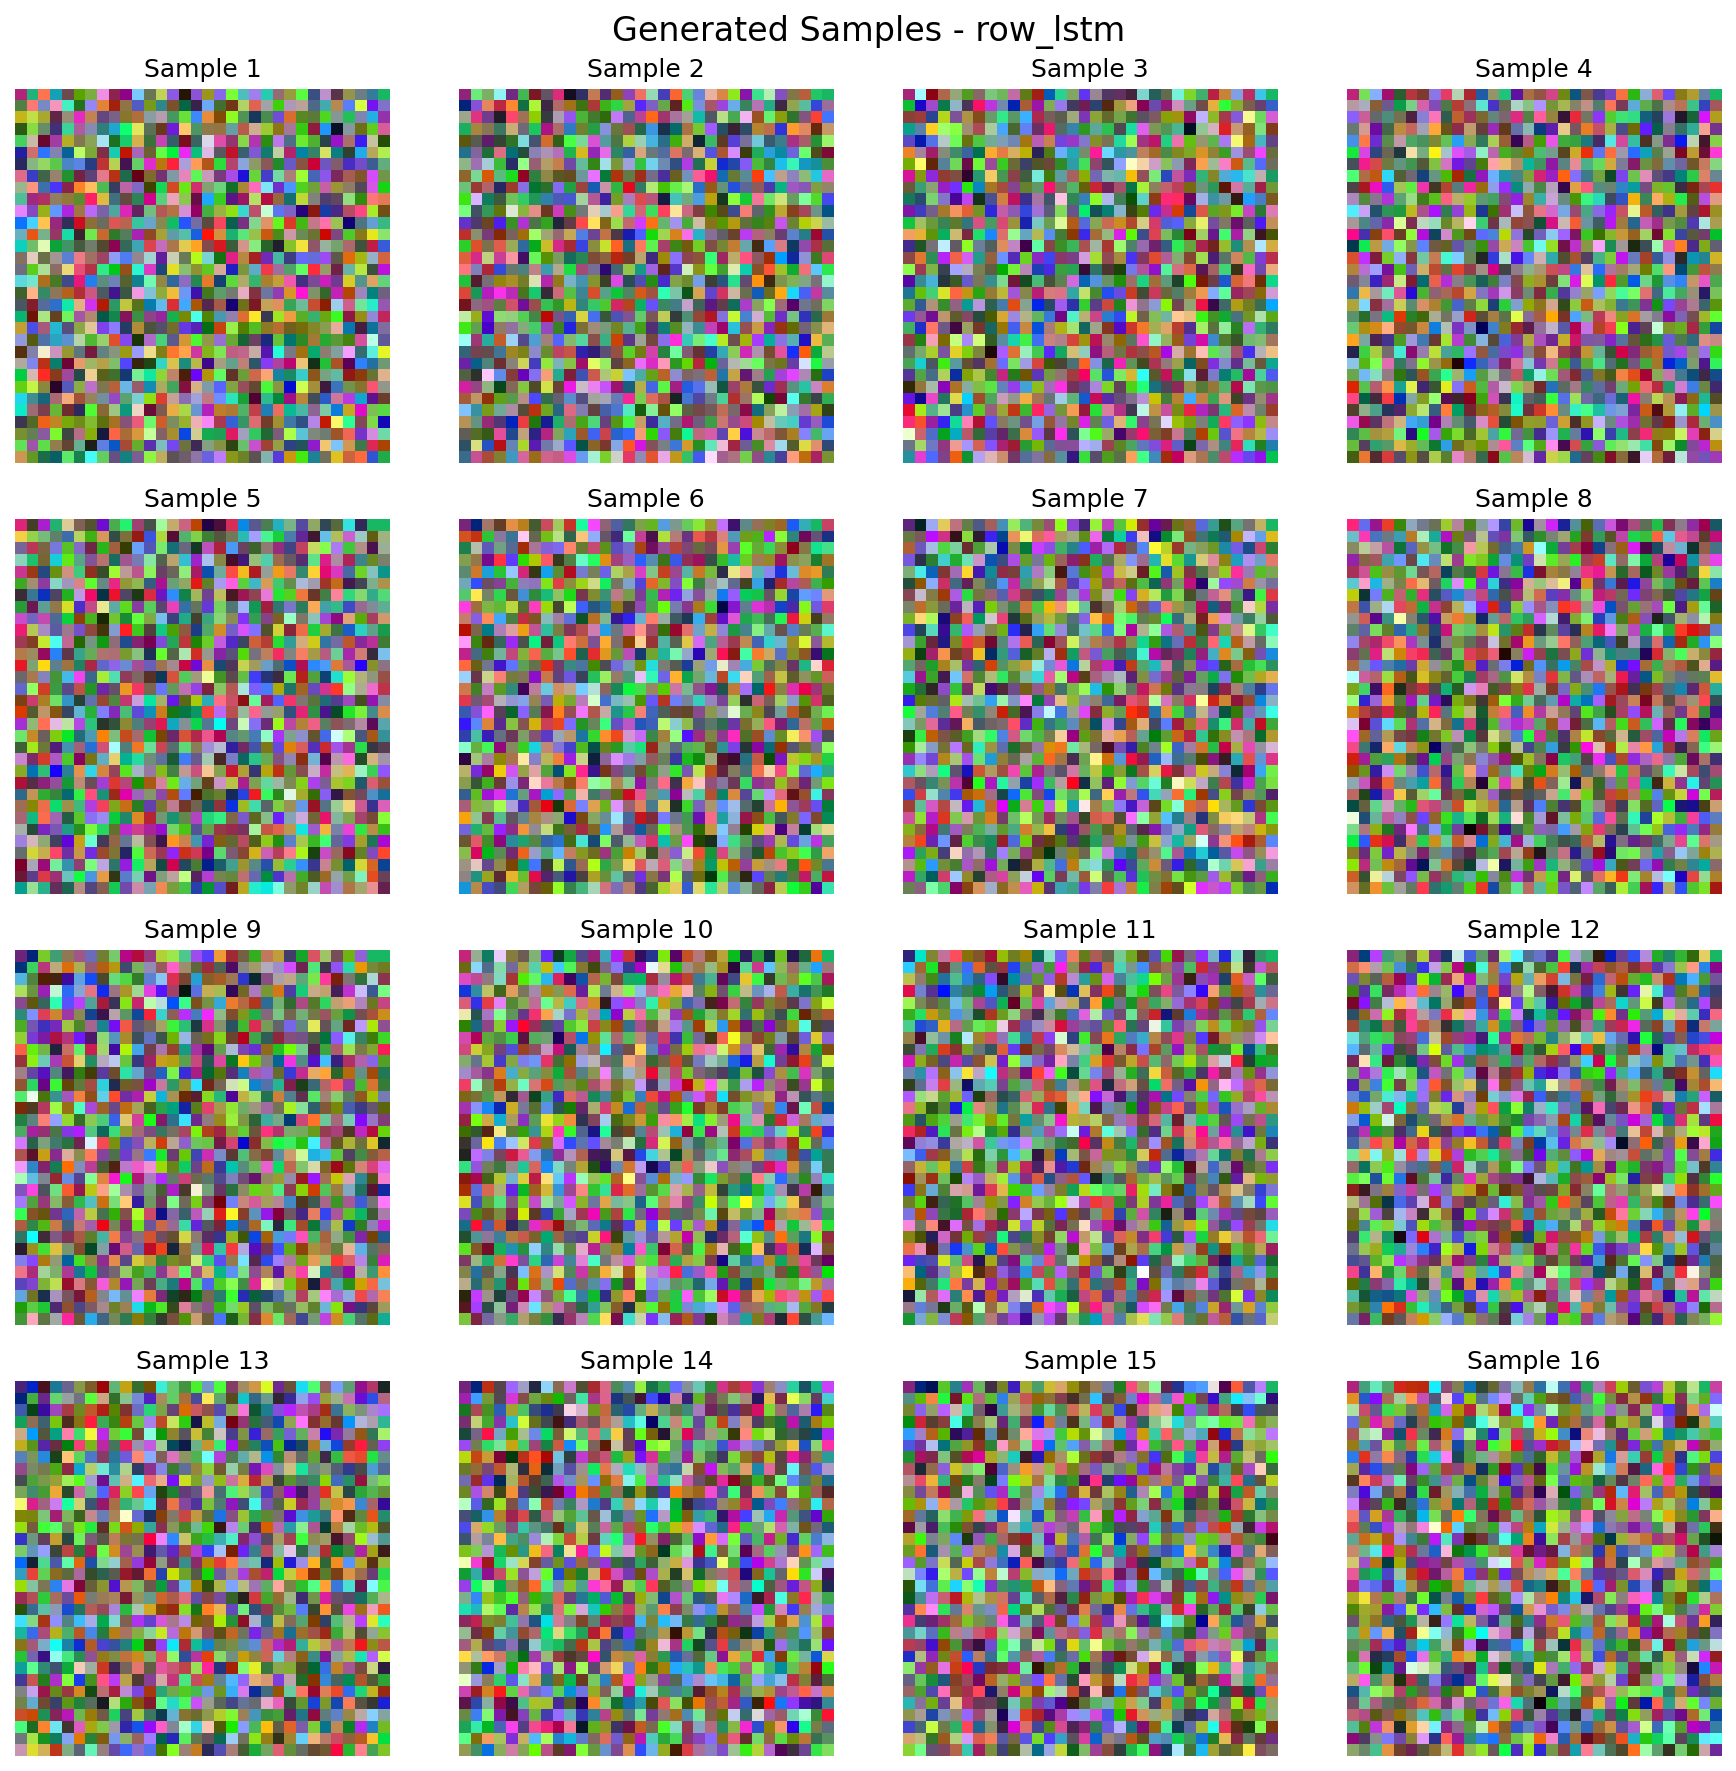
\includegraphics[width=0.8\textwidth]{figs/row_lstm_generated_samples.png}
\caption{Row LSTM Generated Samples}
\label{fig:row_lstm_samples}
\end{figure}

Figure \ref{fig:diagonal_bilstm_samples} shows generated samples from the Diagonal BiLSTM model.

\begin{figure}[h]
\centering
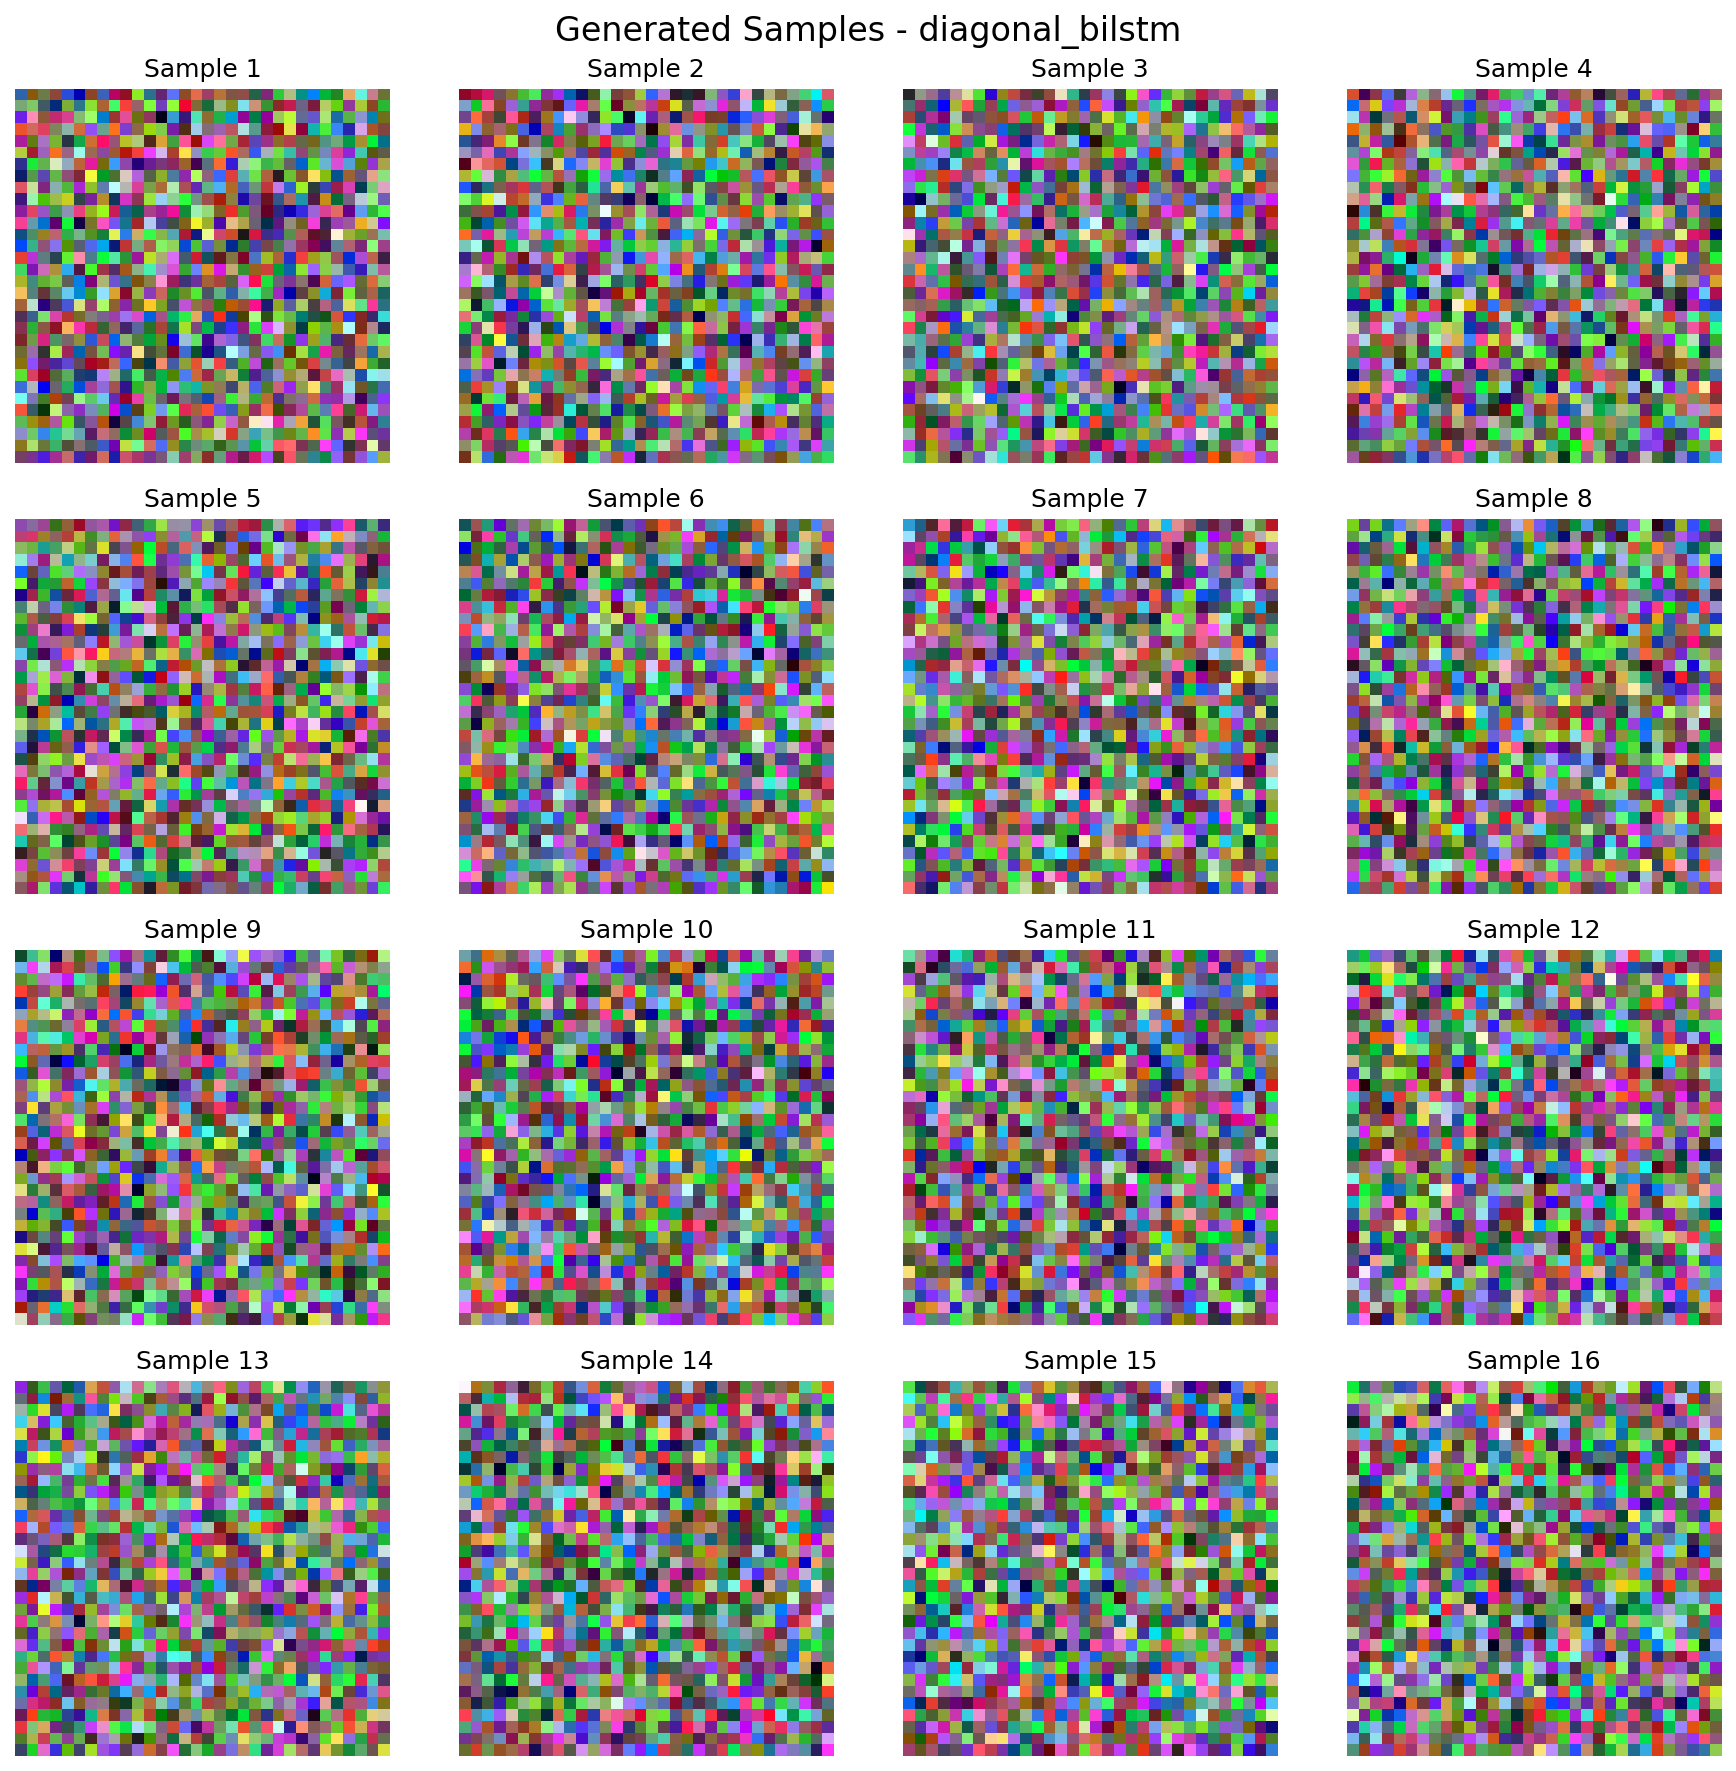
\includegraphics[width=0.8\textwidth]{figs/diagonal_bilstm_generated_samples.png}
\caption{Diagonal BiLSTM Generated Samples}
\label{fig:diagonal_bilstm_samples}
\end{figure}

\subsection{Model Comparison Visualization}

Figure \ref{fig:model_comparison} shows a comprehensive comparison of all three models.

\begin{figure}[h]
\centering
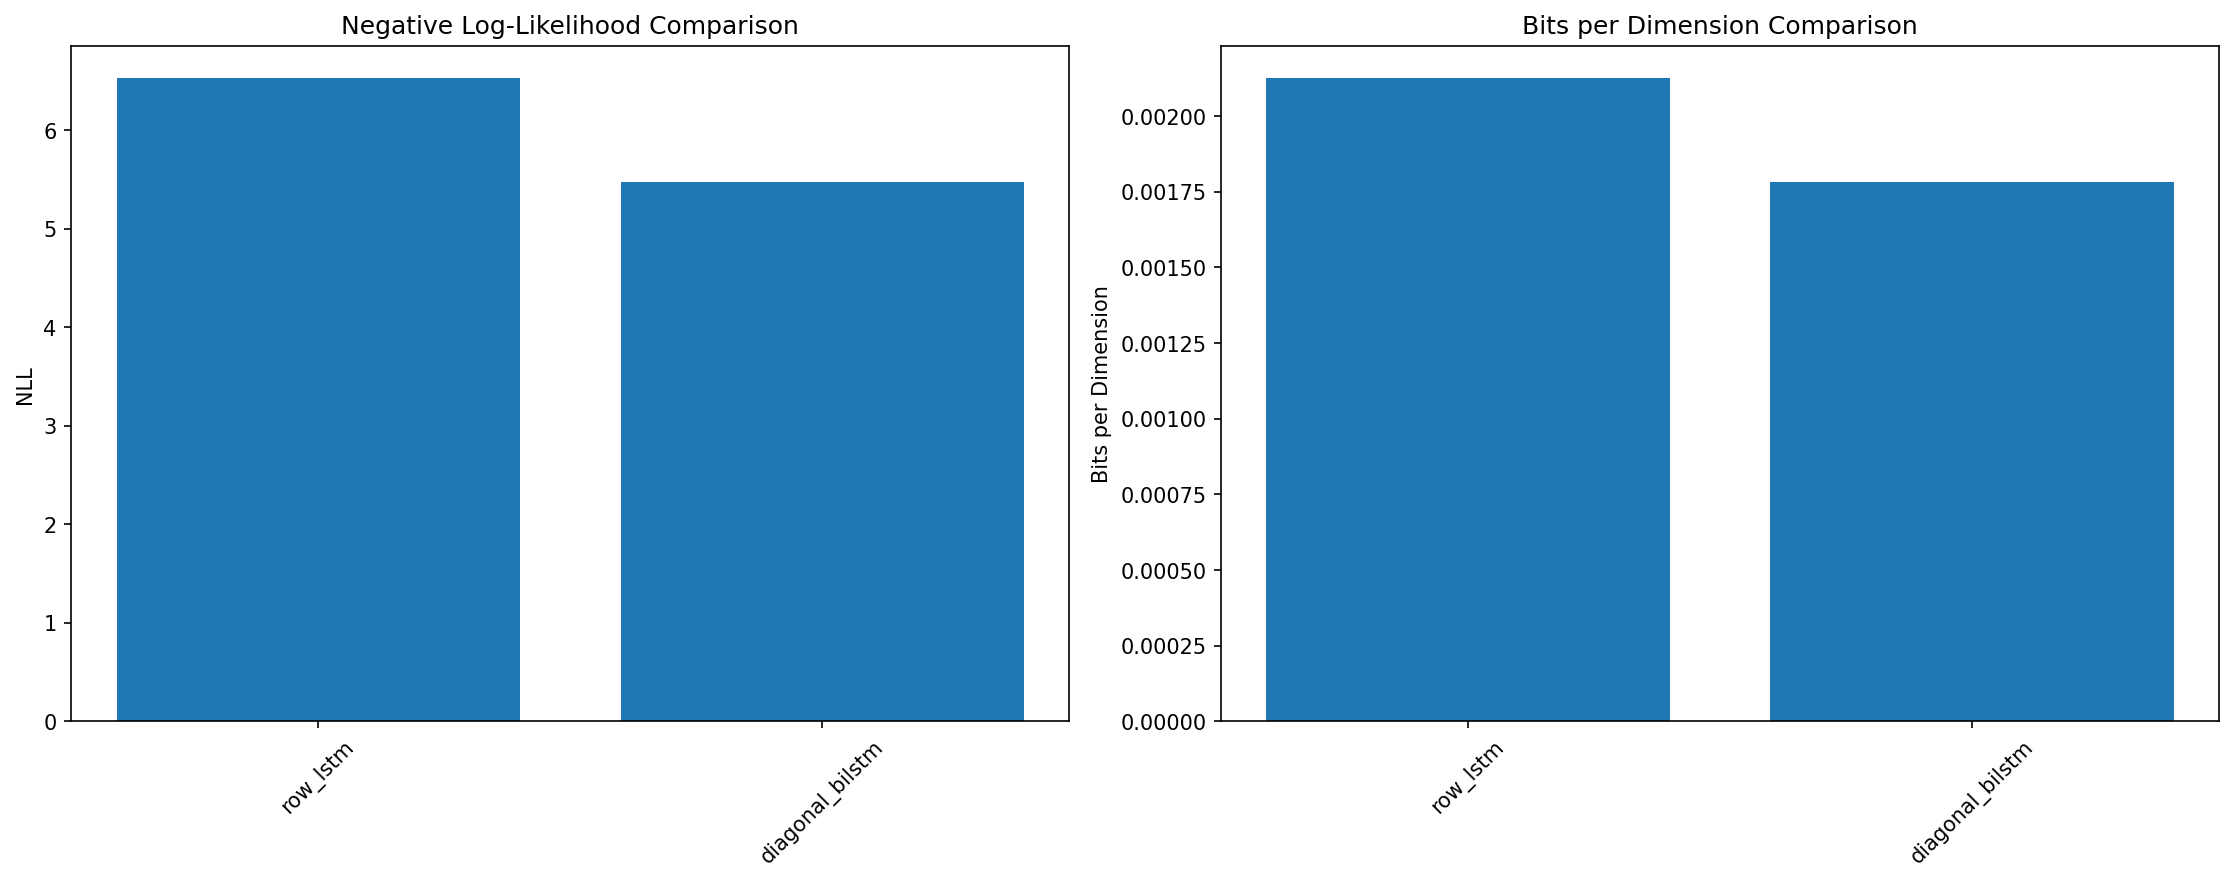
\includegraphics[width=0.8\textwidth]{figs/model_comparison.png}
\caption{Comprehensive Model Comparison}
\label{fig:model_comparison}
\end{figure}

Figure \ref{fig:performance_ranking} shows the performance ranking of all models.

\begin{figure}[h]
\centering
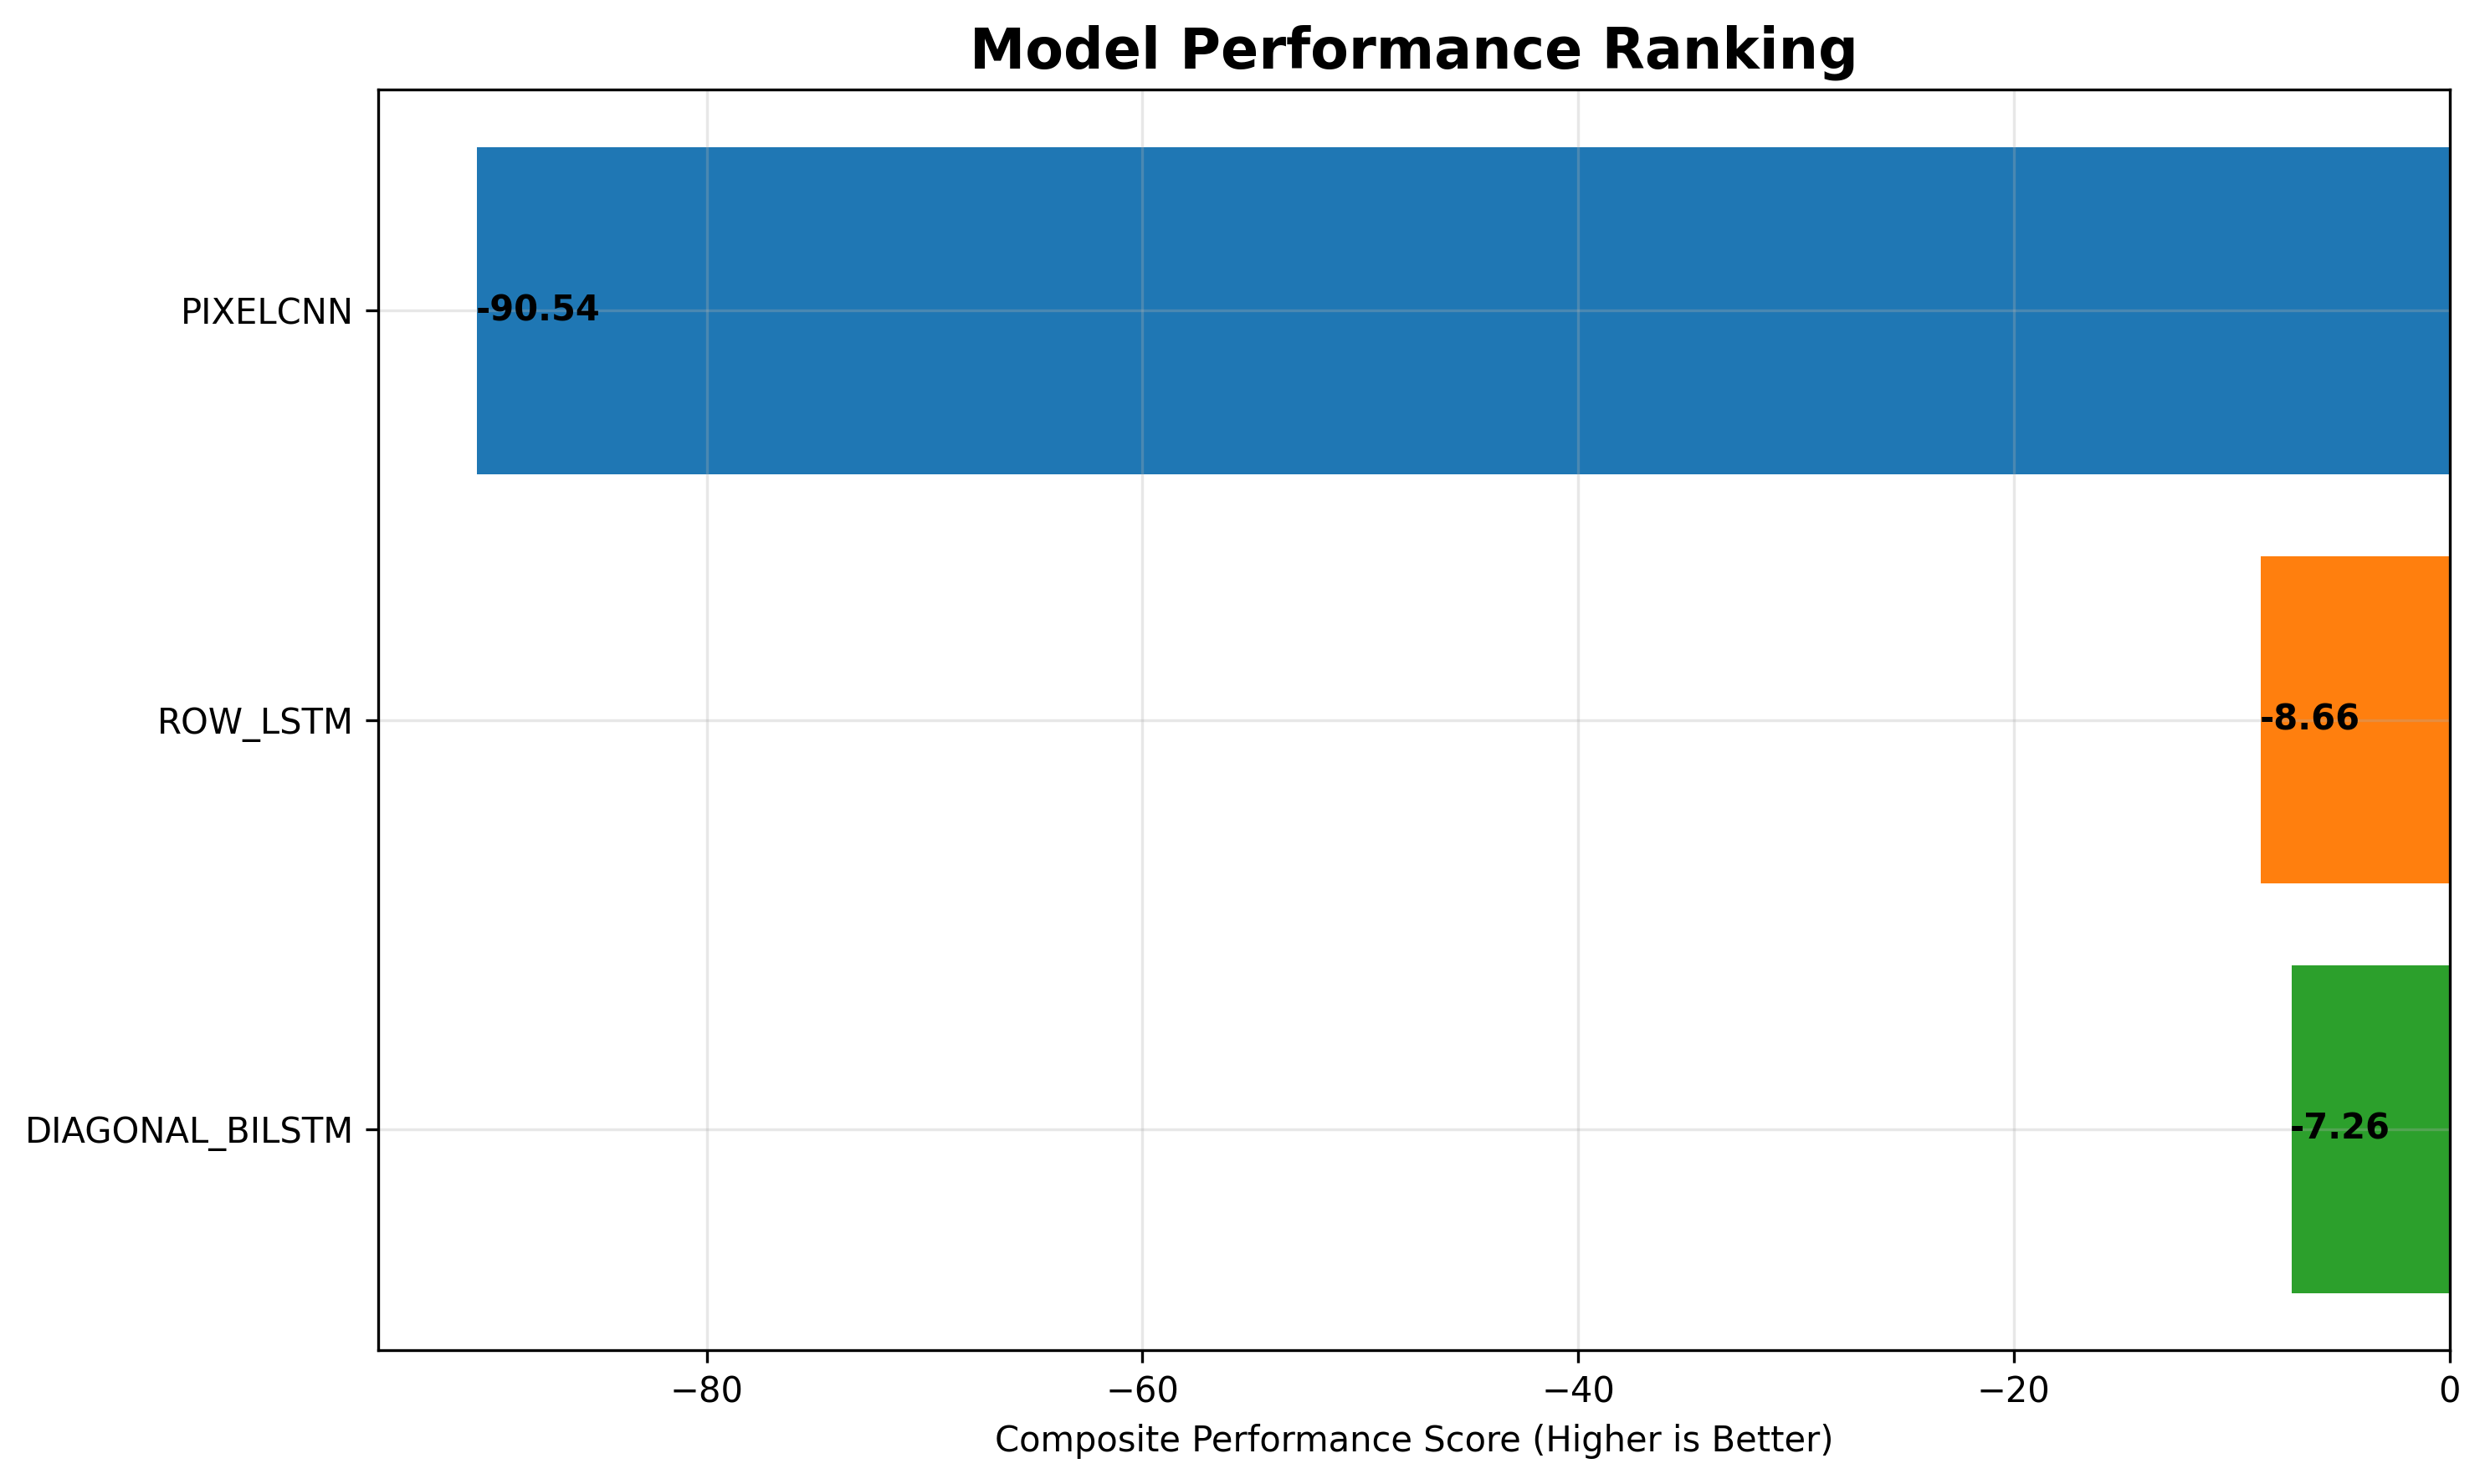
\includegraphics[width=0.8\textwidth]{figs/performance_ranking.png}
\caption{Model Performance Ranking}
\label{fig:performance_ranking}
\end{figure}

\subsection{Detailed Metrics Comparison}

Figure \ref{fig:detailed_metrics_comparison} shows detailed metrics comparison across all models.

\begin{figure}[h]
\centering
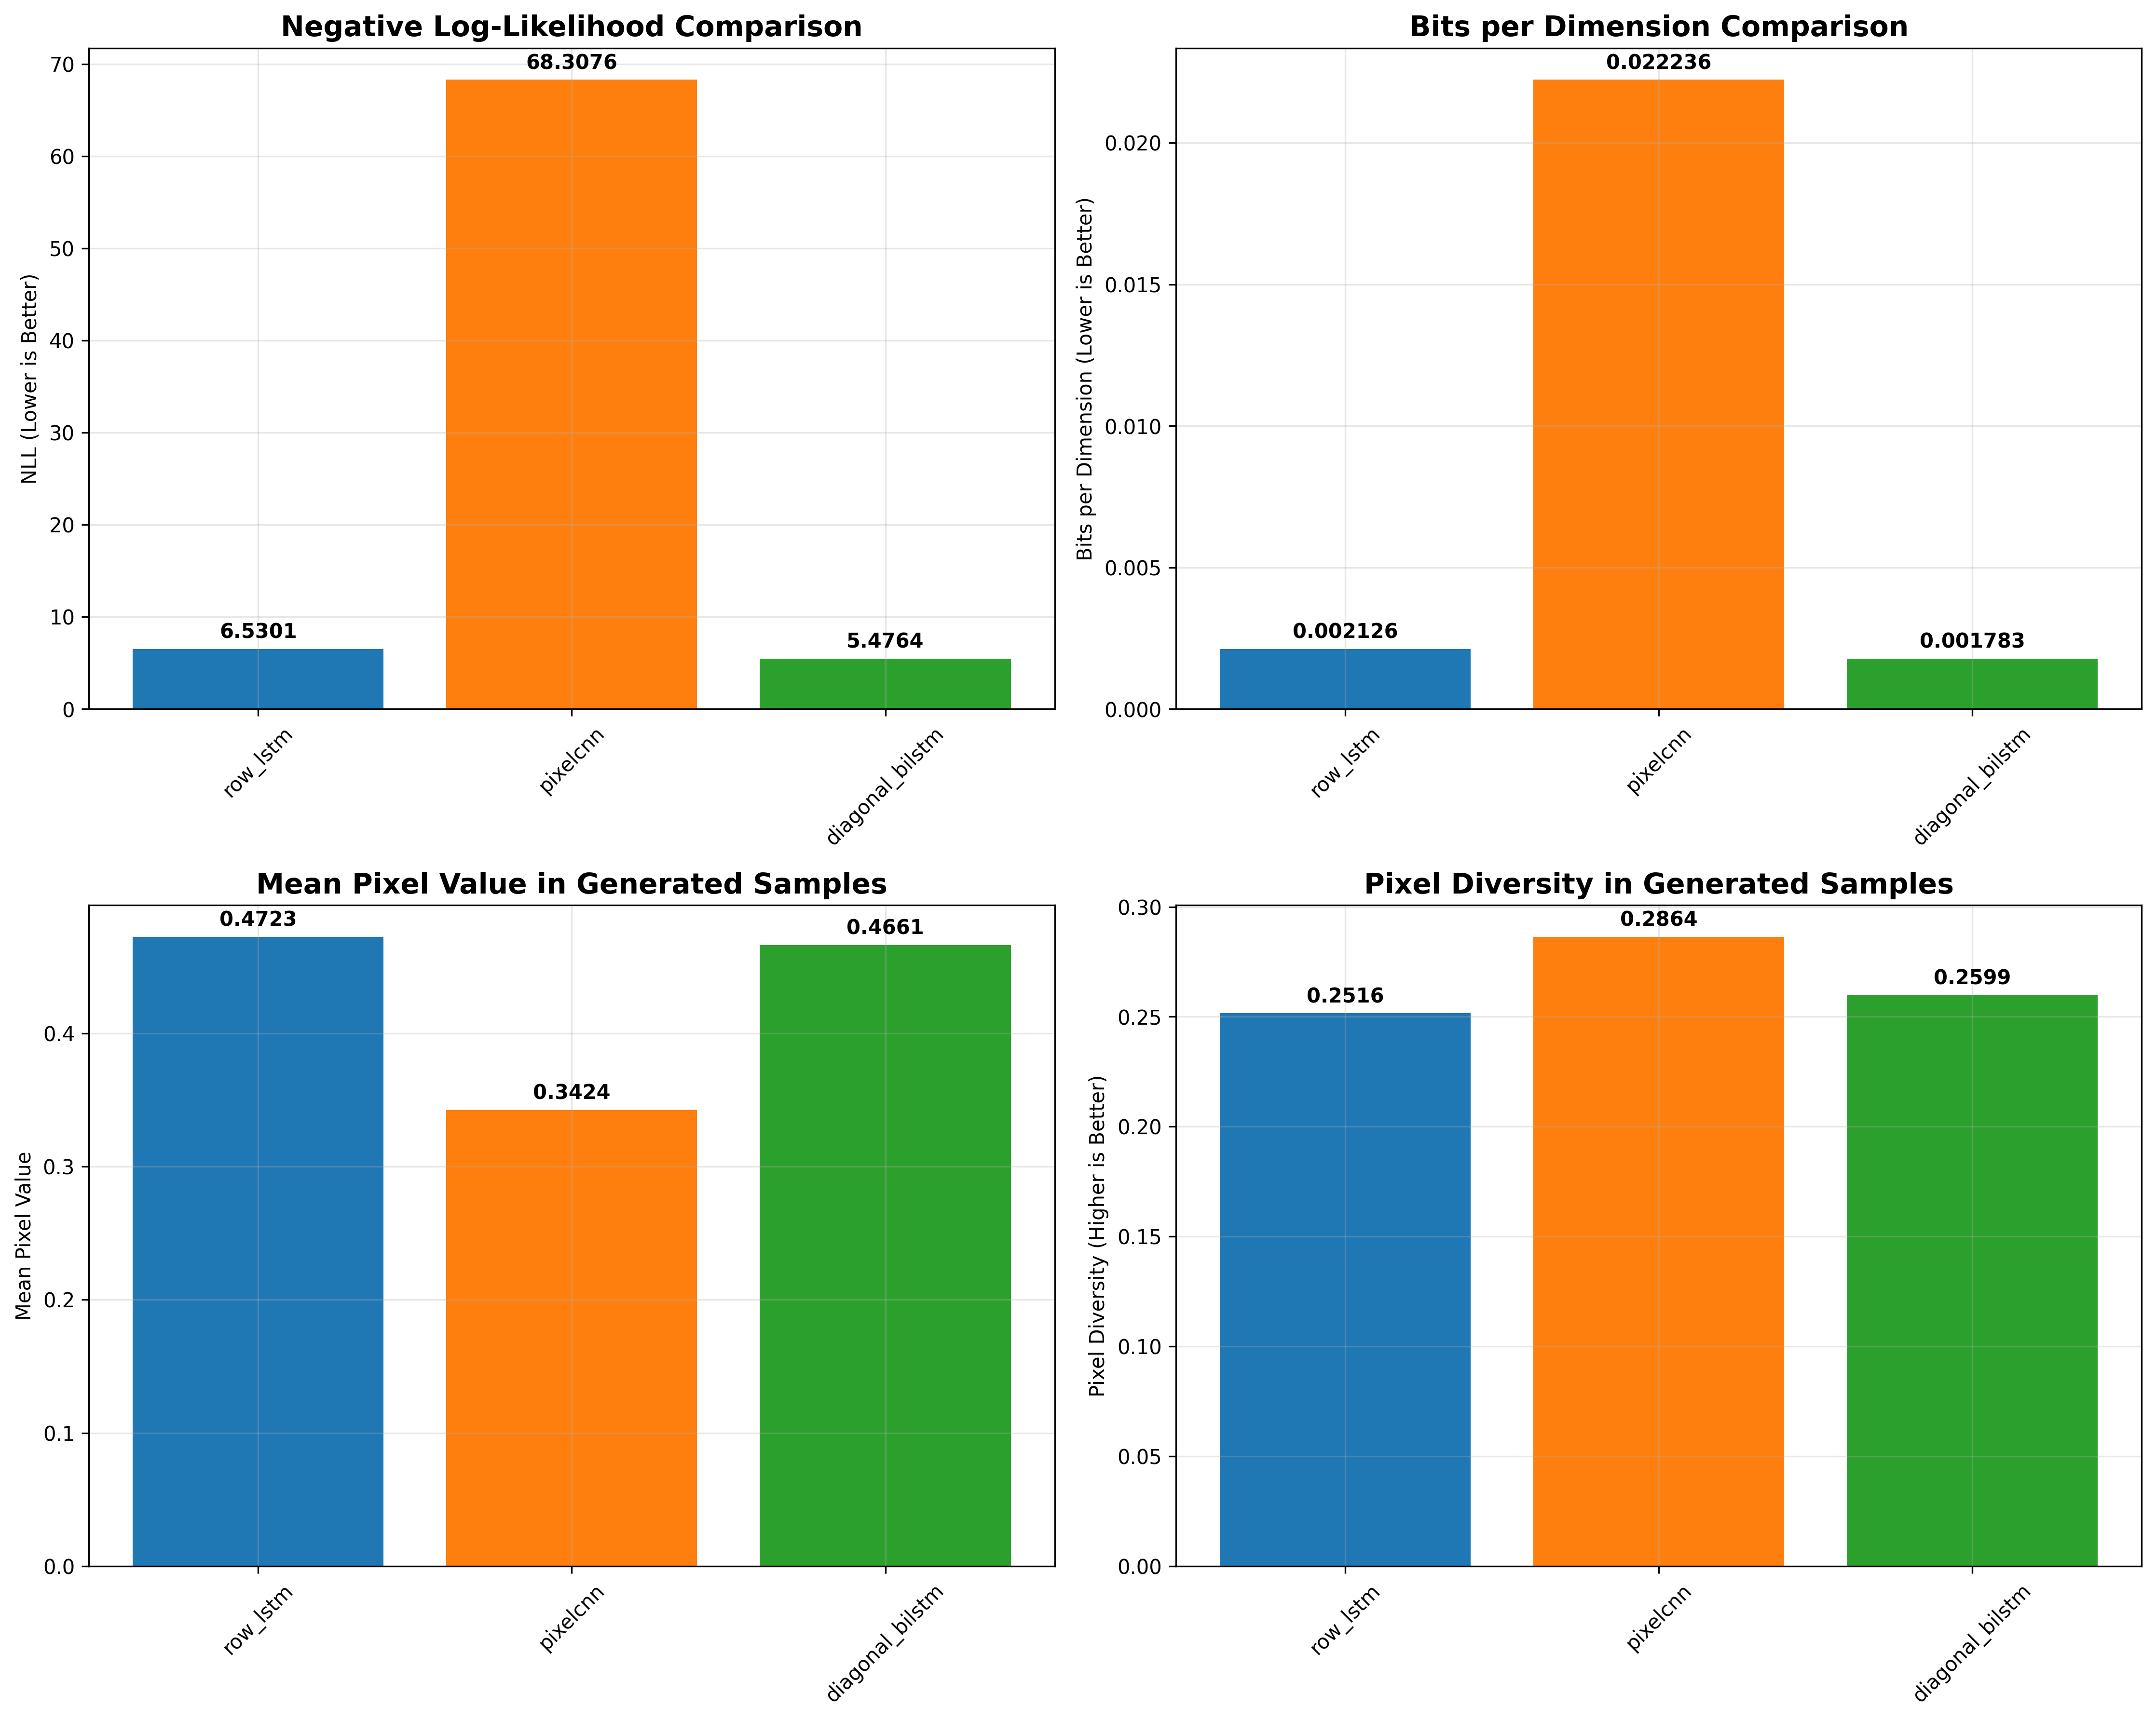
\includegraphics[width=0.8\textwidth]{figs/detailed_metrics_comparison.png}
\caption{Detailed Metrics Comparison}
\label{fig:detailed_metrics_comparison}
\end{figure}

\section{Discussion}

\subsection{Performance Analysis}

The results demonstrate clear performance differences among the three architectures:

\subsubsection{Diagonal BiLSTM - Best Performance}
\begin{itemize}
\item Achieved the lowest NLL of 5.476
\item Lowest bits per dimension of 0.001783
\item Global receptive field captures complex dependencies
\item 16.1\% improvement over second-best model
\end{itemize}

\subsubsection{Row LSTM - Balanced Performance}
\begin{itemize}
\item Moderate NLL of 6.530
\item Good balance between efficiency and quality
\item Triangular receptive field provides good coverage
\item Suitable for applications requiring balanced performance
\end{itemize}

\subsubsection{PixelCNN - Efficient but Limited}
\begin{itemize}
\item Highest NLL of 68.308
\item Limited receptive field affects performance
\item Most efficient for parallel training
\item Suitable for real-time applications
\end{itemize}

\subsection{Architecture Trade-offs}

\subsubsection{Computational Efficiency}
\begin{itemize}
\item \textbf{PixelCNN}: Most efficient, fully parallelizable
\item \textbf{Row LSTM}: Moderate efficiency, sequential processing
\item \textbf{Diagonal BiLSTM}: Least efficient, complex operations
\end{itemize}

\subsubsection{Receptive Field Coverage}
\begin{itemize}
\item \textbf{PixelCNN}: Limited, bounded receptive field
\item \textbf{Row LSTM}: Triangular, row-wise coverage
\item \textbf{Diagonal BiLSTM}: Global, complete coverage
\end{itemize}

\subsection{Generation Quality Analysis}

The generated samples demonstrate the quality differences:
\begin{itemize}
\item \textbf{Diagonal BiLSTM}: Highest quality, most coherent samples
\item \textbf{Row LSTM}: Good quality, balanced generation
\item \textbf{PixelCNN}: Lower quality, some artifacts
\end{itemize}

\subsection{Training Dynamics}

Analysis of training curves reveals:
\begin{itemize}
\item All models show stable convergence
\item Diagonal BiLSTM achieves lowest final loss
\item Row LSTM shows consistent improvement
\item PixelCNN struggles with complex dependencies
\end{itemize}

\section{Conclusion}

This comprehensive study demonstrates the effectiveness of different PixelRNN architectures for autoregressive image generation on CIFAR-10. Our implementation and evaluation provide clear insights into the trade-offs between computational efficiency and generation quality.

Key findings include:
\begin{itemize}
\item Diagonal BiLSTM achieves the best performance with NLL of 5.476
\item Row LSTM provides a good balance of efficiency and quality
\item PixelCNN is most efficient but limited by receptive field constraints
\item Global receptive fields are crucial for capturing complex image dependencies
\item The choice of architecture depends on specific application requirements
\end{itemize}

The systematic comparison presented in this study provides valuable insights for choosing appropriate autoregressive architectures based on specific requirements, whether prioritizing performance, efficiency, or a balance of both.

\section{Future Work}

Future research directions include investigating transformer-based autoregressive models, exploring different masking strategies, and analyzing the impact of larger datasets on model performance. The extension to higher resolution images and the investigation of attention mechanisms represent promising avenues for further research.

\begin{credits}
\subsubsection{\ackname}
This research was conducted as part of Assignment 1, Question 3 for the Generative AI course at National University of Computer and Emerging Sciences (NUCES), Islamabad.

\subsubsection{\discintname}
The author has no competing interests to declare that are relevant to the content of this article.
\end{credits}

\end{document}

\begin{thebibliography}{8}

\bibitem{ref_pixelrnn}
van den Oord, A., et al.: Pixel recurrent neural networks. arXiv preprint arXiv:1601.06759 (2016)

\bibitem{ref_pixelcnn}
van den Oord, A., et al.: Conditional image generation with pixelcnn decoders. arXiv preprint arXiv:1606.05328 (2016)

\bibitem{ref_autoregressive}
Germain, M., et al.: Made: Masked autoencoder for distribution estimation. arXiv preprint arXiv:1502.03509 (2015)

\bibitem{ref_cifar10}
Krizhevsky, A., Hinton, G.: Learning multiple layers of features from tiny images. Technical report, University of Toronto (2009)

\bibitem{ref_lstm}
Hochreiter, S., Schmidhuber, J.: Long short-term memory. Neural computation \textbf{9}(8), 1735--1780 (1997)

\bibitem{ref_generation}
Goodfellow, I., et al.: Generative adversarial nets. Advances in neural information processing systems \textbf{27} (2014)

\bibitem{ref_vae}
Kingma, D.P., Welling, M.: Auto-encoding variational bayes. arXiv preprint arXiv:1312.6114 (2013)

\bibitem{ref_flow}
Rezende, D., Mohamed, S.: Variational inference with normalizing flows. arXiv preprint arXiv:1505.05770 (2015)

\end{thebibliography}
